\documentclass{article}
\usepackage{xeCJK}
\author{Richard Gendal Brown, James Carlyle, Ian Grigg, Mike Hearn}
\date{2016年8月}
\title{Corda:介紹}
%%\setlength{\parskip}{\baselineskip}
\usepackage{amsfonts}
\usepackage{listings}
\usepackage{color}
\usepackage{epigraph}
\usepackage{graphicx}
\graphicspath{ {images/} }
\usepackage[export]{adjustbox}
\usepackage{float}
\usepackage{hyperref}
\usepackage[super,comma,sort&compress]{natbib}
\usepackage[nottoc]{tocbibind}
%\usepackage[natbibapa]{apacite}
\renewcommand{\thefootnote}{\alph{footnote}}
%\epigraphfontsize{\small\itshape}
\setlength\epigraphwidth{4.5cm}
\setlength\epigraphrule{0pt}
\begin{document}
\maketitle 
\begin{abstract}
由相互不信任的節點組成的分佈式帳本讓單一的全球資料庫得以產生,其記錄機構和人員之間的交易和責任狀態。這不但大大消除目前將獨立帳本相互同步而所花的人力及時間,還可以提升目前金融業使用的代碼分享等級,從而為大家降低金融服務成本。我們向您介紹 Corda,一個為滿足這些目標而設計的平台。本文為一般讀者作全面的介紹。即將出版的技術白皮書會進一步說明設計和基礎建構決策。
\end{abstract}
\newpage
\tableofcontents
\newpage
\section{介紹}
在 R3,我們相信分佈式帳本技術具有使金融服務業脫胎換骨的潛力,並使其客戶及類似的參與公司受益。我們預見未來的金融合約可以記錄無誤及自動管理,而且任何人可以在毫無爭議的情況下就任何合約目的順暢執行交易。我們相信市場走向的模式是,涉及金融合約的各對象將記錄金融合約一次,並在保持這些合約準確及分享紀錄上相互合作。重複紀錄、對帳、無法配對、斷裂等問題將會成為過去。孤立的資產表述將不復再。

我們渴望為金融服務使用案例定出一個共享的帳本結構,可憑藉成熟的技術在現有的法律框架內實施。我們的理念可以分為三類:機構要求的工程、專注於非功能需求和可擴展性。

我們相信本文介紹的 Corda 平台設計特點對受監管的金融機構來說是吸引的選擇。\footnote{可以透過以下電子郵件聯絡本文作者:Richard Gendal Brown \href{mailto:richard@r3cev.com}{(richard@r3cev.com)}、James Carlyle \href{mailto:james@r3cev.com}{(james@r3cev.com)}、Ian Grigg \href{mailto:iang@r3cev.com}{(iang@r3cev.com)}、Mike Hearn \href{mailto:mike@r3cev.com}{(mike@r3cev.com)}}

\section{主文}
銀行是其中一批最早開始使用資訊科技的採納者,並且與大眾的普遍看法相違背,他們在過去將人工流程自動化及實體流程數位化等方面做的非常好。然而,可見的建構在成本以及效率上仍存在很多改善的機會。 

特別是,每間金融機構都有自己的分類帳,以記錄該公司對客戶群和對手的合約和立場的看法。反之,其對手也保持自己的看法。此類重複紀錄可能會導致出現不協調,並且各對象需要對一項交易進行昂貴的配對、對帳及修改錯誤。兩家公司對同一宗交易的看法存在差異也是風險的來源,而且其中一些還可能涉及系統性風險。

金融機構的多重性會產生競爭及選擇,但其依賴的科技平台的多重性則會造成複雜及營運風險。然而,直到最近,這是不可避免的:除了集中市場基礎設施補充說明{這方面的例子包括美國證券集中保管結算公司 (DTCC) 以及持續連結清算集團 (CLS)。}之外,只有少數的有效方法能夠在不整合企業本身的前提下整合公司間的科技。

集中市場基礎設施公用事業已朝著增加公司間的資料及業務邏輯分享的方向發展,但整體而言,其在金融交易領域達到的整合程度仍遠遠落後於網絡出現以來在資訊交換領域取得的成就。\cite{IT}

我們相信,加密技術的成熟,比如說特別是通常稱為「區塊鍊技術」的部分,提供了一個新的機會,即是公司間能安全分享權威紀錄系統的可能性。這一項願景透過使用新分享平台記錄財務事件及處理業務邏輯,提供改造金融公司的經濟機會,特別是但不限於交易後服務的機會;即是一個權威的單一全球邏輯分帳,並適用於公司間在分帳記錄的所有合約。這個建構將為這個行業定出一個新的共享平台,讓現存者、新進入者及第三方均可爭相提供創新的產品及服務。 

\begin{figure}[H]
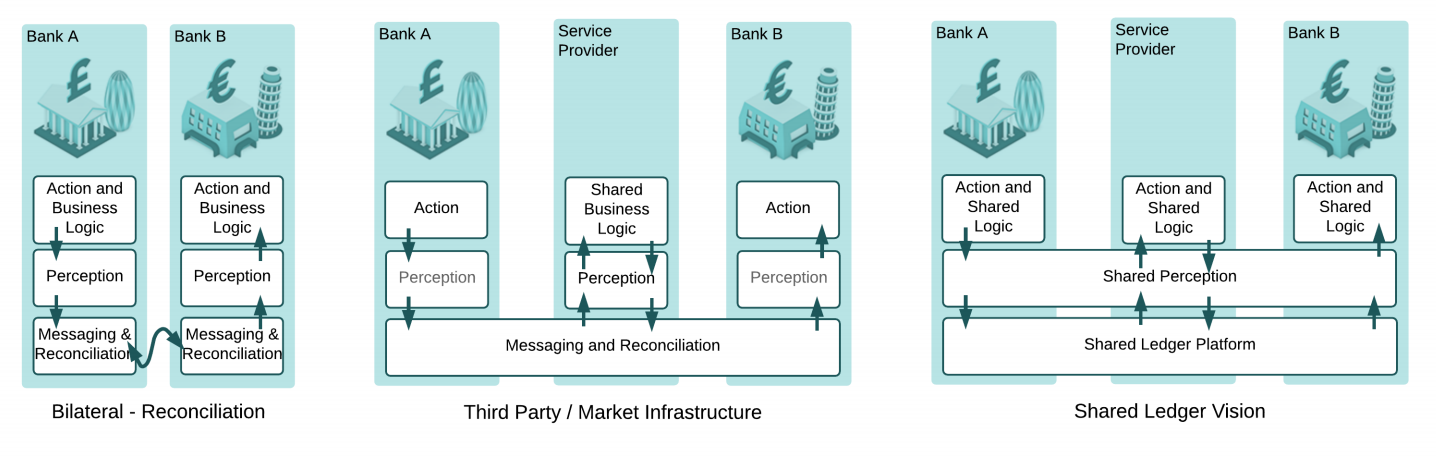
\includegraphics[scale=.5, center]{sharedlogic} 
\caption{在上圖中,我們展示從各對象分享個別記錄事實及管理本身紀錄,以及其相關連的差異和重複 (\textit{「雙方 – 對帳」}) 的世界,或各方將關鍵流程的控制及責任委任給集中式公用事業 (\textit{「第三方/市場基礎建設」}) 的世界,進展成為一個相互合作維持共享紀錄、確保一致協調,並 在開放及競爭的基礎上使用現存及新服務供應商和市場基礎建設提供者所提供的服務 (\textit{「共享帳本的願景」})。}
\end{figure}


我們相信,從較高質素的資料、較少的差異,以及各公司之間更快速同意各項細節所節省下來的費用將甚為可觀。此外,在各個公司間裝置此通用建構將會定出一個新平台,讓現有及新供應商可爭相滿足客戶的需求。再者,使用不同系統記錄同一宗交易細節也是產生成本及複雜的主要源頭。因此,該平台也可能在公司內部應用。

\section{願景}
長遠而言,可以預見一個「全球邏輯帳本」,讓所有的經濟行動者進行互動,並且任何對象均可以使用安全、一致、可靠、私人及權威的方式記錄及管理彼此之間的合約。我們所說的全球性,是指每個人就屬於他們的資料所看到的內容均相同,而邏輯性是指實際的執行可能會以不同的方式組成。因此,一個可能出現的最終狀態將是,我們從公司內部保留的權威系統記錄轉移到公司\textit{間}分享的全球權威系統紀錄。 

\subsection{最終狀態原理}
使用分佈式帳本技術可能導致的最終狀態的背後原理可能包含:
\begin{itemize}
	\item 依照合約,由帳本記錄的事實在任何爭議中均可被接受為可使用的證據並且對各對象均存在法律約束力。
	\item 由帳本記錄的事實被視為權威,而非其他地方的權威數據的「影子」,因此,和解能在平台上直接進行。
	\item 一旦合約經由相關的各個對象同意,帳本上紀錄的事實即為最終且不可變的;錯誤及逆向交易均必須透過後續交易處理。公司將面臨重新設計內部流程以提高準繩和質量的壓力。
	\item 任何行動者在原則上均得以與帳本直接連結,並用其記錄與對手的合約。任何行動者均不會被迫與他人執行交易,但我們可以預期看到「層級」或分級市場模式的遞減。 
	\item 透過推廣開放式標準及包容式存取,現有及新的服務提供商均可連結及爭相提供不同的服務,從而促進選擇和競爭。
	\item 應能獲得金融交易細節的唯一對象是當事人本人及合法需要知悉的其他人。
\end{itemize}

然而,該願景包含了過渡期狀態的概念,例如首先側重於商業邏輯共享的概念。這是為了承認今日的系統在可預見的未來仍會持續伴隨我們的事實,解決方案的設計將需要以共存、整合及遷移路徑等部分作為基礎。這些過渡期狀態在長期願景的法律和其他非技術性問題另行得到解決的同時亦可以產生相當的價值。

應該強調的是,全球邏輯帳本的長期願景旨在為努力的方向定調,但它可能會以多種帳本的形式實現。它可能會為每個資產類別設計一個帳本的形式實現,並且具備自主性及零散耦合的特色,從而在不同的商業服務之間提供功能及營運獨立性。 

願景背後的建構和策略選擇包括:
\begin{itemize} 
\item 此系統管理的紀錄僅能由對其管理的資產及合約具有合法利益的行動者存取。
\item 由系統管理的合約作用將以電腦代碼描述,該代碼會明確引用豐富完整的法律文體,並從中取得合法性。\cite{Ricardian}
\item 為了確定出現合約違約情況,將會為合約代碼升級及爭議解決流程的明確參考提供支援。這是因為即使在自動化設置中,技術和人為因素均會導致合約糾紛。 
\item 此願景將會透過降低成本、風險和監管責任(包括資本、流動性和營運責任),以及透過創新的新產品和服務成功實現。
\item 為了在金融界得到廣泛的採用,系統的一部分必須及將會是開放的:開放原始碼、開放的開發過程、開放式的標準。
\item 即使此願景是以「平台」或「系統」等詞彙稱呼,但我們相信該設計在實際上將會是多層次,可能由不同的供應商透過競爭/合作的方式完成不同的部分。讀者不應假設我們構想的是一個單一的垂直整合方法。
\item 該願景還包括層次堆疊中較高等級的層次可包含各公司或集團的智慧財產專利的可能性。
\item 該系統將在與安全環境對立的假設下運行:日漸增長的網絡犯罪必須被視為不可避免的。
\end{itemize}

我們相信要實現此願景的基礎發明已經存在。這些包含但不限於強效的加密方法、全球通訊網路、定義金融工具的標準,以及有效的演算法以確保實現全球規模等級的一致性。 

讓此願景在今日可能成為現實的原因是近期對分佈式帳本的濃厚興趣,而且區塊鍊系統創造了一個可以公開討論這種願景的環境,況且多個金融機構共同合作的合作聯盟已經形成。它針對網路參與者之間的身份基礎設施進行假設,但不會對其精密複雜或操作模式作出假設。監管參與是設計過程的一項關鍵要素。

根據我們針對現有的分佈式帳本平台進行的需求分析和評估,我們認為現有的平台均無法滿足我們的需求。在本質上,傳統分佈式資料庫設計背後的威脅模式不適用於我們令相互不信任的法律實體達成共識的使用案例,而現存區塊鍊系統的架構則不適用於我們在個別法律合約層面上對限制及謹慎指定的資料分享要求。因此,我們設計並開始開發 Corda。

\section{Corda}
Corda 是一個分佈式帳本平台,用於記錄及處理金融合約,旨在實施本文描述的願景。  

Corda 平台支援智能合約,配合 Clack、Bakshi、Braine 的定義。\cite{SCT} 我們的智能合約是一種在執行上能夠透過電腦代碼\textit{自動化}執行,並能在人工輸入及控制下執行的合約,而且如法律文體所述,其權利及責任在法律上\textit{是有效的}。這項智能合約能將業務邏輯及業務數據與相關連的法律文體連結,以確保平台上的金融合約在法律的角度上牢不可破並且可以執行,並使我們在出現歧義、不確定或爭議時能隨著清楚的道路執行。

\subsection{主要功能}
Corda 是專門為受監管的金融機構而設。它主要受到區塊錬系統的啟發,但卻沒有傳統區塊鍊系統不適用於許多金融狀況的設計選擇。 

Corda 提供了一個利用這些關鍵活動及功能來執行智能合約的框架:
\begin{itemize}
    \item{以現有法律結構為基礎、並能與現有及未來出現的法規結合的方式,記錄及管理金融合約的進展,以及兩個或多個可辨識對象之間的其他共享數據}
    \item{在沒有中央控制器的情況下編排公司間的工作流。}
    \item{支援各公司之間在個別交易層面上達成共識,非為全球系統。}
    \item{支援監管及監督觀察員節點的納入。}
    \item{僅在與交易有關的對象之間驗證交易。}
    \item{支援各種共識機制。}
    \item{記錄人類語言的法律文體文件及智能合約代碼之間的明確連結。}
    \item{使用符合業界標準的工具。}
    \item{限制合約的數據存取權限,僅能由明確授權或邏輯上具有特權權限的使用者存取。}
\end{itemize}
這些功能對設計適用於複雜金融服務組織的平台產生了貢獻。請注意,此設計不使用本機加密電子貨幣或施加執行全球交易限速。

\subsection{概念}
我們是從全球帳本的想法出發:一個可靠的單一來源。然而,在我們的模組中,交易及帳本條目並非所有人都能看見。在交易只涉及對象中的一小部分子群組的情況下,我們會努力將相關數據純粹保留在該子群組中。 

我們概念中的基礎對象是一個\textit{狀態對象},它是一份數位文件,記錄兩個或多個對象之間存在的協議內容及目前狀態。它旨在僅與有正當理由檢視的人士分享。為了確保全球共享系統的一致性,但又不讓參與者檢視所有的數據,我們主要依賴安全密碼雜湊來辨識各個對象及數據。帳本被定義為一組不可變狀態的對象。

我們針對合約的狀態反覆的討論及思考,目標是要確保與合約有關的各對象在合約演變時能維持共識。有人可能會說這就是區塊鍊概念的本質:確保不同行動者持有的數據在更新時能保持一致,並且為可信賴交易奠定基礎:從簡單的貨幣支付到複雜的智能合約轉換。

\begin{figure}[H]
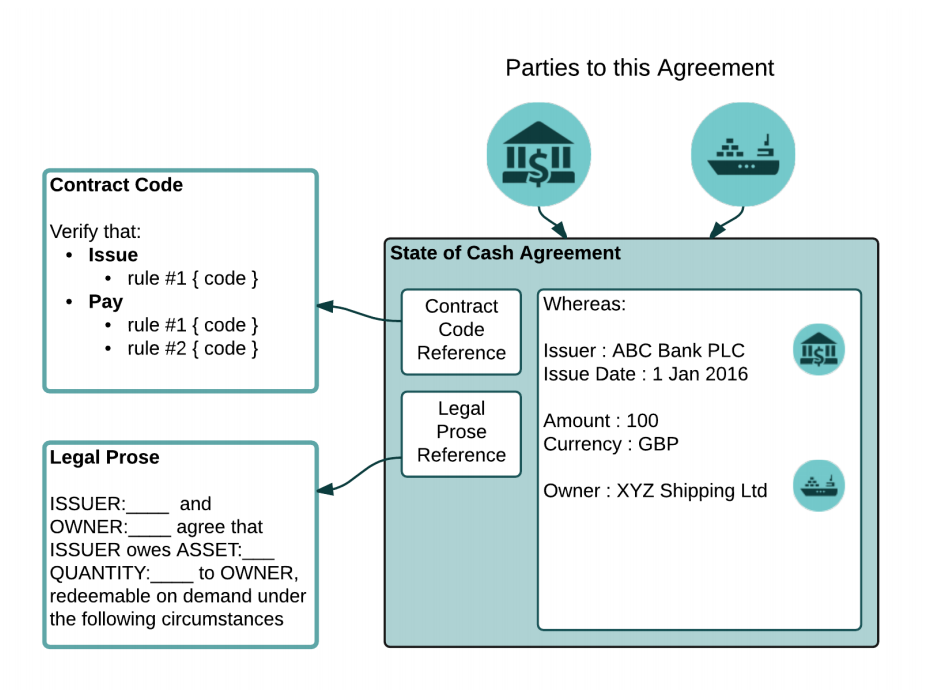
\includegraphics[scale = .4, center]{partiesto}
\caption{在上列的圖表中,我們可以看到一個狀態對象,其代表一個虛構的貨運公司向商業銀行請款現金 100 英鎊。該狀態對象清楚透過雜湊引用其適用的法律文體,及監管其轉換的合約代碼。}
\end{figure}

我們對合約狀態的關注是與系統產生對比,其中,參與者必須取得共識的數據是整個帳本的狀態或整個虛擬機的狀態。Corda 提供了三種主要工具來達成全球分佈式共識:
\begin{itemize}
    \item 根據預先約定規則的智能合約邏輯來確保狀態轉換是有效的。
    \item 唯一性及時間戳服務為交易按照時間進行排序並消除抵觸。
    \item 一個刻意建造的框架,簡化不同對象之間編寫複雜多步驟協定的流程。
    \end{itemize}
    
\subsection{共識}
在 Corda,可透過\textit{交易}應用更新,它會消耗現有的狀態對象並產生新的狀態對象。共識有兩個方面:
\begin{enumerate}
\item{交易有效性:各對象可以透過檢查相關的合約代碼是否運行成功,以及是否具備所有必須的簽章,來確定提議的定義輸出狀態的更新交易是否有效;以及本交易引用的任何交易是否一樣有效。}
\item{交易唯一性:各對象可以確定有疑問的交易是否為其輸入狀態唯一的消費者。即是:在我們過去達成共識(有效性及唯一性)的交易中不存在任何其他消耗相同狀態的交易。}
\end{enumerate}

各對象可以通過獨立運行相同的合約代碼和驗證邏輯來同意交易的有效性。然而,如要在唯一性上達成共識則需要一位預定的觀察者,在許多情況下,會要求獨立的觀察者。

\begin{figure}[H]
    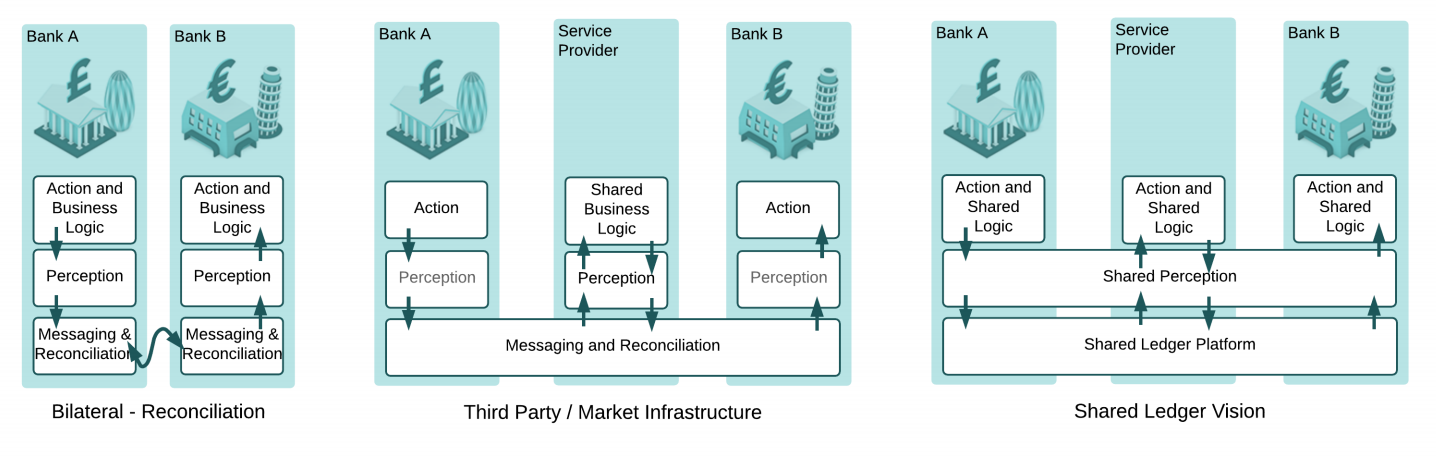
\includegraphics[scale = .5, center]{sharedlogic}
    \caption{交易有效性的共識僅能由與有疑問的交易相關的對象執行。因此,數據只能與需要查看的那些對象分享。其他平台一般在帳本層面上即達成共識。因此,Corda 系統的任何一位行動者僅能看到整個系統管理的整體數據的子集。如果至少兩位行動者對一份數據的存在及細節達成共識,我們將其稱之為「帳本上」,並且允許任意組合的行動者參與任何數據的達成共識流程。僅由一位行動者持有的數據稱為「帳本下」。}
\end{figure}

Corda 擁有「可拔除的」唯一性服務。這是為了提高隱私性、可擴展性、法律制度兼容性\cite{EUC}以及算法敏捷性。一向單一的服務可能會透過拜占庭錯誤容忍算法由許多相互不信任的節點組成,或可能會非常簡單,像是一 部單一的機器。在某些情況下,比如演化一個狀態,會需要所有相關對象的簽章,可能會完全不需要唯一性服務。 

要注意的是,這些唯一性服務僅僅是為了證明特定交易所消耗的狀態是否在過去曾被消耗;它們不需要證明交易本身的有效性,那是屬於與交易有關的各個對象的範疇。這意味著唯一性服務不需要(並且在一般情況下不會)查看任何交易的全部內容,與替代的分佈式帳本及區塊鍊設計相比,這將會顯著提高系統的隱私和可擴展性。此設計決策代表了對共享帳本建構中可接受的取捨重要選擇,並會在未來的技術白皮書中更全面地探討。

\subsection{業務邏輯}
Corda 通過智能合約代碼實施業務邏輯,該代碼被構造為接受或拒絕交易的純函數,並且可以由更簡單、可重複使用的函數組成。這些函數將交易解釋為擷取狀態作為輸入,並透過指令(智能合約)的應用,產生輸出狀態,如果所提議的操作有效,則接受交易。合約定義了帳本的一部份業務邏輯,並且是可移動的:即使我們認為 Corda 部署的簽署代碼會在受監管的環境中使用,但節點將會在沙盒內下載並運行合約,而且不會在某些部署中進行任何審查。 

我們為合約的執行及驗證所選擇的虛擬機是 Java 虛擬機\cite{JVM},因為它擁有豐富的現有資料庫和龐大的技術基礎,並且重新使用行業的標準將會使銀行更容易重新使用現有合約內的代碼。然而,我們使用了定製的沙盒來為其擴增,該定製的沙盒比一般的 JVM 沙盒具有更多限制,它不僅實現了安全性要求,還實現了確定性執行。如同以太坊\cite{以太坊},將Bytecode而非語言進行標準化的選擇,讓使用者可以在合約語言設計中進行創新,或依照喜好重複使用廣泛應用的語言。一旦合約經過審閱,這也使得直接從內部應用程式使用合約代碼變得容易,從而大大地簡化應用程式的開發。

\subsection{核心金融概念}
Corda 的建構深受三個對\textit{建構具有重大意義的使用案例}的影響,並認為是極有可能出現的常見問題的代表。這三個使用案例分別為:現金、安全性工具及衍生性合約。我們認為這三種使用案例都是金融合約的範例:
\begin{itemize}
\item 現金餘額(例如:「下列銀行及我雙方同意,該銀行欠我一百萬美元」)。
\item 受託管的證券(例如:「以下託管銀行與我雙方同意,我擁有下列公司 1,000 股的股票」)。
\item 雙邊衍生合約(例如:「A 銀行和 B 銀行同意他們是以下利率互換(IRS)的當事人,這意味著他們同意在預定的時間,以同意的支付公式交換下列現金流量(淨值)」 )。
\end{itemize}
舉其中一個範例做說明,Corda 的現金設計明確模擬商業現實中不存在「穩操勝算」的事實,只存在一位持有人對指定機構具有的現金請款。\cite{BOE} 因此我們的核心現金合約非常簡單,卻非常的強而有力:我們記錄現金發行人的法定身份、貨幣、金額、所有者(以及其他與請款性質相關的資訊,並明確地指出與管理合約有關的\textit{法律文體} ,在有爭議的情況下我們預期這將具體說明解決流程),並使用這些資訊建立所有其他與現金相關的概念(付款、淨額結算等)。
\begin{figure}[H]

\includegraphics[scale = .4, center]{cash}
\caption{在上列圖表中,我們檢視了 Corda 最簡單的交易之一:一個發行交易。我們看到一個商業銀行向虛構的貨運公司發行了一個新的現金狀態。發行的交易是由發行的銀行簽屬。從這個簡單的模型,可以建構更複雜的交易,例如付款、貨銀對付制度合約及未來日期的責任。}
\end{figure}
\subsection{Corda 模型總結}
我們的模型的核心概念是:
\begin{itemize}
\item \textit{狀態對象}, 代表兩個或多個對象之間的合約,由可透過機器閱讀的\textit{合約代碼}管理。該代碼引用並旨在實施人類可讀的\textit{法律文體}的一部分。\item \textit{交易},在生命週期中轉換狀態對象
\item \textit{交易協定} 或 \textit{業務工作流},讓各個對象可以在不存在中央控制器下協調行動。
\end{itemize}

透過允許選擇性及決定性限制的程式設計技巧,以最大程度提升決定論及將共享狀態數量需求減到最小。

狀態對象(數據)、合約代碼(容許操作)、交易協定(業務邏輯編排)、任何必需的 API、錢包外掛程式,以及 UI 組件的組合可以是一個共享帳本應用程式,或 Corda 分佈式應用程式 (\textit{「CorDapp」})。這是一位平台合約開發人員應預期建造的核心組件。 

%\begin{figure}[H!]
%\includegraphics[scale = .4, center]{image4}
%\caption{Corda 驅動的生態系統中的應用程式的當前想法。}
%\label{fig:figure4}
%\end{figure}

%\begin{figure}[H!]
%\includegraphics[scale = .25, center]{image5}
%\caption{另一個 Corda 將會如何與金融生態系統互動的視覺表象。}
%\label{fig:figure5}
%\end{figure}

\section{與其他平台的比較}
Corda 是與金融從業者廣泛合作建立的,並且根據他們的要求而設計。然而,其設計亦受到過去努力的啟發,其中包含 Todd Boyle 及 Ian Grigg 在三重記帳法\cite{Triple}著作中介紹的內容,以及現存的分佈式帳本平台,比如比特幣\cite{Bitcoin}和以太坊。因此,對於不熟悉 Corda 的人來說,透過這些平台可能更容易理解。 

\subsection{與比特幣的比較}
Corda 與比特幣有著一些顯著的相似之處: 
\begin{itemize}
\item{由交易所消除及建立的不可變的狀態是相同的。}
\item{交易有多個輸入和輸出。比特幣有時將帳本稱為未用的交易輸出集(UTXO 集)。}
\item{合約是一個純粹的功能;合約沒有存儲或與任何事務互動的能力。只要是相同的交易,一份合約的「驗證」功能能總是產生完全相同的結果。}
\end{itemize}

然而,除了比特幣的數量及相關的支出規則(腳本)外,比特幣交易具有單一、固定的數據格式,並且只能容納很少的數據。已經有人嘗試在合約代碼中的半標準位置嵌入數據來嘗試解決這個限制,讓數據可以透過規律配對進行截取,但這不是一種好的方法。相比之下,我們的狀態可以包括任意型態的數據。此外,我們的交易不僅涉及輸入合約,還涉及輸出合約。比特幣交易的接受僅受合約代碼中消除的輸入狀態控制。我們使用「合約」一詞來代表一組可以處理不同任務的業務邏輯,其範圍超出交易驗證。舉例來說,我們的合約目前包含建立有效交易的代碼(這在比特幣中經常被稱為「錢包代碼」)。


比特幣腳本只能給出一組固定的字節數組作為輸入。這意味著合約沒有辦法檢查整個交易的結構,這嚴重限制了合約能做的事情。我們的合約是圖靈完整的,並且可以用任何針對 JVM 的普通程式語言編寫。	
Corda 允許在交易中(必須由受信任的時間戳記證明)任意指定精確的時間限制,而不是依賴於區塊被開採的時間點。這點非常重要,因為我們所設想要支援的許多合約類型均需要準確的時間,以及我們的主要共識實施使用了無區塊衝突解決算法。要注意的是,Corda 不使用工作證明或有「挖礦」的概念。

\subsection{與以太坊的比較}
如同以太坊,代碼是在一個相對強大的虛擬機中運行,並且可以包含複雜的邏輯。非組裝程式語言可用於合約編程。它們均是意圖使用於多種不同類型的金融合約模組。

然而,以太坊的「合約」一詞是指由每個參與節點複製和維護程式的舉例說明。此舉例說明與對象導向程式中的對象非常類似:它可以接收和發送消息,更新本地存儲等。相比之下,我們在代碼中的智能合約的實現是指一組功能,僅有其中的一部份是在保持系統同步(\textit{驗證}功能)。該功能是單純且無狀態的(也就是,它在執行時不得與任何其他系統產生互動)。	由於合約沒有任何類型的可變存儲,因此不存在「訊息」的概念。以太坊同時也聲稱不僅僅是一個金融邏輯的平台,而可做各種不同的應用。我們的平台至少在初期不將非金融應用包括在內。

%\section{成功的範例:現金}
%狀態對象(描述的)代表是各個對象之間共享的合約。

%狀態包含了任意數據,但他們總是包含至少一個對合約代碼的雜湊引用。該代碼是一個以字節碼表示的程式,在虛擬機中運行沙盒,以及法律文體文件的雜湊引用,該引用將會以受司法或其他爭議解決制度承認的形式提供法律內容。\textit{合約代碼} (或在本文其餘部分僅稱為合約) 是全球共享的部分業務邏輯資訊。合約總是定義一個驗證函數,這是一個能夠確定狀態轉換是否有效的單純函數,不論哪一對象調用該函數。驗證函數不檢查交易是否符合任一個對象的利益,只檢查其約束被強制執行,並且節點必須在符合自己的利益下單獨滿足自己的交易。這將會在後面有更多的討論。

%在上圖中,我們看到一個風格化的現金狀態對象,代表對 100 美元的所有權。該對象是指其管理合約及相關的法律文體。由於這是一份現金合約,法定文體將具體說明一個對象向另一個對象發行的現金負債所屬的條款和條件:在什麼情況下,現金對象可以在傳統銀行帳戶中兌換餘額,或在其他地方兌換電匯?爭議將會如何得到解決?等等。此外,該法律文體將說明與合約相關的權利、責任及條件,並且各對象將會同意透過電腦代碼進行自動化。我們將明確從法律文體領域委任至代碼領域。

%此外,重要的是,法律文體將留下數個未指定的資訊:誰是發行者及貨幣是什麼?狀態對象中包含了這些欄位(我們看到這裡的發行人是巴克萊銀行,貨幣為美元)。法律文體、合約代碼及狀態對象中擷取的參數加上相關的數位簽章共同界定了各對象之間的合約。

%在下文中,我們將描述如上所述的狀態對象範例能夠如何使用 Corda 建構的其他組件,在各對象之間的演化、處理以及傳輸。

%附註:這類設計在很大的程度上類似於比特幣的「UTXO 模型」。然而,它也有一些顯著的差異。UTXO 風格的模組相對於以太坊使用的帳戶/餘額模組的選擇,是一種有認知及刻意的選擇,並且是平台的隱私和可擴展性特徵的基礎。

\section{路線圖}
為了達到這個設計,我們首先在代碼中模擬並建立 Corda 的組建的原型來驗證這個概念的各個方面。這是一個 Corda 模型的延伸的部份列表(而非全部,並預計將在近期至中期完成。
\begin{itemize}	
\item 交易的分解及唯一性的增強:加入機制來選擇掩蓋部分的交易,包括來自唯一性服務的混淆。
\item 合約驗證沙盒:明確的連結時間將積極的 Java 資料庫的最小集列入白名單。
\item 一個用於位置推斷的插入式錢包。
\item 計算邏輯或閘道至可以被參與者驗證為帳本上的所有權(或其他)業務邏輯執行者(例如:中央交易對手或估價代理人)。
\item	使用 Corda 模型來管理使用者的身份。
\item 互操作性和數據整合,特別是 FpML、ISO20022,支援其他數據格式和與其他平台的整合/互操作性。
\item	為參考數據建立應用程式。
\item	使用地址隨機化、零知識證明、資產重新發行計劃等技術增加隱私性。
\item	為未來的金融工具建立參考合約。
\item 投資組合級業務邏輯的本機支援,例如狀態對象的整合。
\end{itemize}
\section{總結}
與大多數目前現存的分佈式帳本及區塊鍊平台相比,Corda 是在註冊金融機構之間記錄及執行業務合約的明確目的下建立;它不是旨在成為所有問題的通用解決方案。因此,它需要一種獨特的數據分配和交易語義方法,並與此同時維持其最初吸引機構的分佈式帳本功能,比如 R3 的項目等,即是以自動化和可實施的方式可靠執行財務協議。
\bibliographystyle{unsrt}
\bibliography{Ref}

\end{document}
